\section{Evaluation and Benchmarking}\label{sec:evaluation}

Our evaluation centers on a head-to-head token comparison between OraViz and the official Oracle SQLcl MCP server. SQLcl is an appropriate comparator because it is Oracle's shipped CLI with a built-in MCP mode (\texttt{sql -mcp}), it talks to the same database instances as OraViz, and its tool surface (\texttt{run-sql}, \texttt{connect}, \texttt{schema-information}, and supporting tools) covers the same class of database questions. Other official options, such as ORDS-based endpoints and the OCI Database Tools MCP, require service deployments that would confound a token comparison with infrastructure differences, so they are out of scope for this report.

Because the experiments in this report were run under specific server versions, database contents, and tokenizer choices, the reported numbers should be interpreted as measurements of the evaluated configuration rather than universal properties of the two servers. The harness, the data, and the commands to reproduce every number are released with the artifact.

\subsection{Setup}

Both servers point at one Oracle AI Database 26ai Free instance running in a container (version banner 23.26.0), loaded with the demo schema shipped with the artifact: \texttt{SALES\_DEMO}, 96 rows of monthly sales across 12 months, 4 regions, and 2 channels, and \texttt{PRODUCT\_VECTORS}, a small table with an 8-dimensional \texttt{VECTOR} column. The SQLcl MCP server runs from SQLcl 26.1 on Java 21. Both servers execute the same SQL for the query stages.

The harness measures five questions: listing the schema objects; describing \texttt{SALES\_DEMO}; aggregating revenue by region for the last six months; sampling ten rows; and fetching the full 96-row table, which stands in for the unaggregated exploratory query that motivates the contract. Each question is answered with the idiomatic tool of each server: \texttt{list\_tables}, \texttt{get\_table\_schema}, \texttt{execute\_query}, and \texttt{sample\_table\_data} for OraViz, and \texttt{schema-information} plus \texttt{run-sql} for SQLcl. SQLcl's \texttt{connect} tool accepts only saved connections, so connecting goes through \texttt{run-sqlcl} with a connect string; that step is counted separately as SQLcl-only setup because the benchmark must connect before it can ask anything.

\subsection{Metrics}

For a server, the benchmark reports the token cost of its tool schemas $S(\mathcal{T})$, the summed cost of the tool results $\sum_i R_i$, and the total $T = S + \sum_i R_i$ following Equation~\ref{eq:session}. Relative savings for a stage or for the workflow are
\begin{equation}
\text{savings} \;=\; \frac{T_{\text{sqlcl}} - T_{\text{oraviz}}}{T_{\text{sqlcl}}} \times 100\% .
\label{eq:savings}
\end{equation}
Counts are produced with \texttt{tiktoken} \cite{tiktoken2024} using the \texttt{cl100k\_base} encoding, with \texttt{o200k\_base} computed for robustness. Only text blocks are counted; chart images are a different modality and are reported separately. The database is static during the run, so the measurement is deterministic.

\subsection{Results}

Table~\ref{tab:steps} reports the per-question token counts, and Figure~\ref{fig:benchmark-steps} shows the same data. The two discovery-heavy stages and the wide dump favor OraViz by large margins, while the three small-result stages favor SQLcl.

\begin{table}[t]
\centering
\small
\begin{tabular}{lrrr}
\toprule
Question & OraViz tokens & SQLcl tokens & Savings \\
\midrule
list objects & 69 & 354 & 80.5\% \\
describe table & 143 & 93 & $-53.8$\% \\
aggregate revenue by region & 63 & 40 & $-57.5$\% \\
sample 10 rows & 375 & 242 & $-55.0$\% \\
raw 96-row dump & 825 & 2{,}136 & 61.4\% \\
\bottomrule
\end{tabular}
\caption{Per-question token counts (\texttt{cl100k\_base}). Negative savings indicate stages where the official server is denser; these are small result sets whose framing overhead is bounded by the contract.}
\label{tab:steps}
\end{table}

\begin{figure}[t]
  \centering
  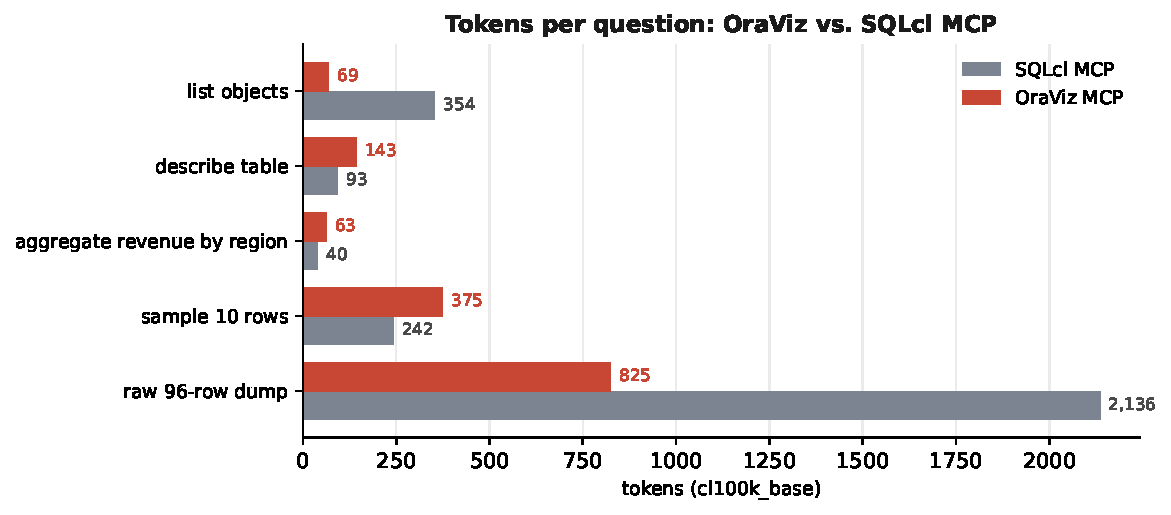
\includegraphics[width=0.92\textwidth]{figures/fig_benchmark_steps.pdf}
  \caption{Tokens per question for the two servers. OraViz wins discovery and wide-result stages by large margins and loses small-result stages; the workflow total is dominated by the former.}
  \label{fig:benchmark-steps}
\end{figure}

Table~\ref{tab:totals} aggregates the workflow. Tool schemas cost $60.5$\% fewer tokens for OraViz, tool results cost $53.7$\% fewer, and the workflow total is $53.7$\% lower, $2{,}319$ tokens against $5{,}006$. Figure~\ref{fig:benchmark-totals} visualizes the budget by stage, and the SQLcl-only connect step adds two tokens that the total accounts for. Under \texttt{o200k\_base} the numbers move by less than one point ($53.6$\% total savings), so the aggregate result is not an artifact of one tokenizer vocabulary.

\begin{table}[t]
\centering
\small
\begin{tabular}{lrrr}
\toprule
Stage & OraViz tokens & SQLcl tokens & Savings \\
\midrule
Tool schemas (once per session) & 844 & 2{,}139 & 60.5\% \\
Tool results (five questions) & 2{,}319 & 5{,}004 & 53.7\% \\
Workflow total & 2{,}319 & 5{,}006 & 53.7\% \\
\bottomrule
\end{tabular}
\caption{Workflow token budget (\texttt{cl100k\_base}). The schema row is a fixed per-session cost; the result rows reflect the contract's effect on every call.}
\label{tab:totals}
\end{table}

\begin{figure}[t]
  \centering
  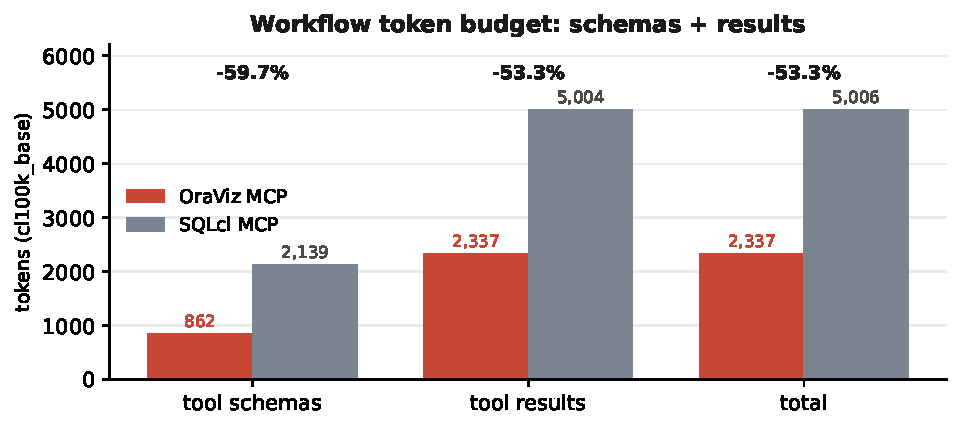
\includegraphics[width=0.92\textwidth]{figures/fig_benchmark_totals.pdf}
  \caption{Token budget by stage. The savings are largest where context would otherwise grow: tool schemas paid up front, discovery, and wide result sets.}
  \label{fig:benchmark-totals}
\end{figure}

\subsection{Estimated token behavior of the chart path}

Rendering the aggregate query of the workflow as a bar chart costs $123$ text tokens plus a single PNG image, which replaces the tabulated result for the comparison question. SQLcl MCP has no chart tool, so the stage cannot be compared directly; the relevant observation is that the text-side cost of the visual answer is independent of the underlying row count, consistent with Equation~\ref{eq:chart}, while the tabular alternative scales with the number of rows the agent chooses to inspect.

\subsection{Analysis}

Three observations follow from the tables. First, the largest savings come from schema discovery: SQLcl's \texttt{schema-information} answers a broader question than ``which tables exist'', returning indexes, LOB segments, sequences, and a DDL outline, and the agent pays for all of it ($354$ tokens against $69$). The comparison is therefore generous to SQLcl only in the sense that it delivers strictly more output; for the question actually asked, the extra output is overhead.

Second, the contract shifts cost from the data to the budget: the raw $96$-row dump costs $61.4$\% fewer tokens because the preview cap renders $25$ rows with an explicit truncation marker, and the cost of that result is the same whether the table has $96$, $96{,}000$, or $96$ million rows. The official server's cost grows with the table, so the measured gap widens with data size.

Third, the losses are real and bounded. Markdown framing (header, divider, padding) costs roughly $55$\% more than CSV on tiny payloads such as a ten-row sample, but that overhead is a function of the column count and the caps, not of the row count, so it cannot grow with the data. The aggregate result is $53.7$\% fewer tokens, with the residual risk of a small, fixed premium on very small answers.
